\documentclass[]{article}
\usepackage{lmodern}
\usepackage{amssymb,amsmath}
\usepackage{ifxetex,ifluatex}
\usepackage{fixltx2e} % provides \textsubscript
\ifnum 0\ifxetex 1\fi\ifluatex 1\fi=0 % if pdftex
  \usepackage[T1]{fontenc}
  \usepackage[utf8]{inputenc}
\else % if luatex or xelatex
  \ifxetex
    \usepackage{mathspec}
  \else
    \usepackage{fontspec}
  \fi
  \defaultfontfeatures{Ligatures=TeX,Scale=MatchLowercase}
\fi
% use upquote if available, for straight quotes in verbatim environments
\IfFileExists{upquote.sty}{\usepackage{upquote}}{}
% use microtype if available
\IfFileExists{microtype.sty}{%
\usepackage{microtype}
\UseMicrotypeSet[protrusion]{basicmath} % disable protrusion for tt fonts
}{}
\usepackage[margin=1in]{geometry}
\usepackage{hyperref}
\hypersetup{unicode=true,
            pdftitle={Social-ecological network dynamics},
            pdfborder={0 0 0},
            breaklinks=true}
\urlstyle{same}  % don't use monospace font for urls
\usepackage{color}
\usepackage{fancyvrb}
\newcommand{\VerbBar}{|}
\newcommand{\VERB}{\Verb[commandchars=\\\{\}]}
\DefineVerbatimEnvironment{Highlighting}{Verbatim}{commandchars=\\\{\}}
% Add ',fontsize=\small' for more characters per line
\usepackage{framed}
\definecolor{shadecolor}{RGB}{248,248,248}
\newenvironment{Shaded}{\begin{snugshade}}{\end{snugshade}}
\newcommand{\KeywordTok}[1]{\textcolor[rgb]{0.13,0.29,0.53}{\textbf{{#1}}}}
\newcommand{\DataTypeTok}[1]{\textcolor[rgb]{0.13,0.29,0.53}{{#1}}}
\newcommand{\DecValTok}[1]{\textcolor[rgb]{0.00,0.00,0.81}{{#1}}}
\newcommand{\BaseNTok}[1]{\textcolor[rgb]{0.00,0.00,0.81}{{#1}}}
\newcommand{\FloatTok}[1]{\textcolor[rgb]{0.00,0.00,0.81}{{#1}}}
\newcommand{\ConstantTok}[1]{\textcolor[rgb]{0.00,0.00,0.00}{{#1}}}
\newcommand{\CharTok}[1]{\textcolor[rgb]{0.31,0.60,0.02}{{#1}}}
\newcommand{\SpecialCharTok}[1]{\textcolor[rgb]{0.00,0.00,0.00}{{#1}}}
\newcommand{\StringTok}[1]{\textcolor[rgb]{0.31,0.60,0.02}{{#1}}}
\newcommand{\VerbatimStringTok}[1]{\textcolor[rgb]{0.31,0.60,0.02}{{#1}}}
\newcommand{\SpecialStringTok}[1]{\textcolor[rgb]{0.31,0.60,0.02}{{#1}}}
\newcommand{\ImportTok}[1]{{#1}}
\newcommand{\CommentTok}[1]{\textcolor[rgb]{0.56,0.35,0.01}{\textit{{#1}}}}
\newcommand{\DocumentationTok}[1]{\textcolor[rgb]{0.56,0.35,0.01}{\textbf{\textit{{#1}}}}}
\newcommand{\AnnotationTok}[1]{\textcolor[rgb]{0.56,0.35,0.01}{\textbf{\textit{{#1}}}}}
\newcommand{\CommentVarTok}[1]{\textcolor[rgb]{0.56,0.35,0.01}{\textbf{\textit{{#1}}}}}
\newcommand{\OtherTok}[1]{\textcolor[rgb]{0.56,0.35,0.01}{{#1}}}
\newcommand{\FunctionTok}[1]{\textcolor[rgb]{0.00,0.00,0.00}{{#1}}}
\newcommand{\VariableTok}[1]{\textcolor[rgb]{0.00,0.00,0.00}{{#1}}}
\newcommand{\ControlFlowTok}[1]{\textcolor[rgb]{0.13,0.29,0.53}{\textbf{{#1}}}}
\newcommand{\OperatorTok}[1]{\textcolor[rgb]{0.81,0.36,0.00}{\textbf{{#1}}}}
\newcommand{\BuiltInTok}[1]{{#1}}
\newcommand{\ExtensionTok}[1]{{#1}}
\newcommand{\PreprocessorTok}[1]{\textcolor[rgb]{0.56,0.35,0.01}{\textit{{#1}}}}
\newcommand{\AttributeTok}[1]{\textcolor[rgb]{0.77,0.63,0.00}{{#1}}}
\newcommand{\RegionMarkerTok}[1]{{#1}}
\newcommand{\InformationTok}[1]{\textcolor[rgb]{0.56,0.35,0.01}{\textbf{\textit{{#1}}}}}
\newcommand{\WarningTok}[1]{\textcolor[rgb]{0.56,0.35,0.01}{\textbf{\textit{{#1}}}}}
\newcommand{\AlertTok}[1]{\textcolor[rgb]{0.94,0.16,0.16}{{#1}}}
\newcommand{\ErrorTok}[1]{\textcolor[rgb]{0.64,0.00,0.00}{\textbf{{#1}}}}
\newcommand{\NormalTok}[1]{{#1}}
\usepackage{graphicx,grffile}
\makeatletter
\def\maxwidth{\ifdim\Gin@nat@width>\linewidth\linewidth\else\Gin@nat@width\fi}
\def\maxheight{\ifdim\Gin@nat@height>\textheight\textheight\else\Gin@nat@height\fi}
\makeatother
% Scale images if necessary, so that they will not overflow the page
% margins by default, and it is still possible to overwrite the defaults
% using explicit options in \includegraphics[width, height, ...]{}
\setkeys{Gin}{width=\maxwidth,height=\maxheight,keepaspectratio}
\IfFileExists{parskip.sty}{%
\usepackage{parskip}
}{% else
\setlength{\parindent}{0pt}
\setlength{\parskip}{6pt plus 2pt minus 1pt}
}
\setlength{\emergencystretch}{3em}  % prevent overfull lines
\providecommand{\tightlist}{%
  \setlength{\itemsep}{0pt}\setlength{\parskip}{0pt}}
\setcounter{secnumdepth}{0}
% Redefines (sub)paragraphs to behave more like sections
\ifx\paragraph\undefined\else
\let\oldparagraph\paragraph
\renewcommand{\paragraph}[1]{\oldparagraph{#1}\mbox{}}
\fi
\ifx\subparagraph\undefined\else
\let\oldsubparagraph\subparagraph
\renewcommand{\subparagraph}[1]{\oldsubparagraph{#1}\mbox{}}
\fi

%%% Use protect on footnotes to avoid problems with footnotes in titles
\let\rmarkdownfootnote\footnote%
\def\footnote{\protect\rmarkdownfootnote}

%%% Change title format to be more compact
\usepackage{titling}

% Create subtitle command for use in maketitle
\newcommand{\subtitle}[1]{
  \posttitle{
    \begin{center}\large#1\end{center}
    }
}

\setlength{\droptitle}{-2em}
  \title{Social-ecological network dynamics}
  \pretitle{\vspace{\droptitle}\centering\huge}
  \posttitle{\par}
  \author{}
  \preauthor{}\postauthor{}
  \date{}
  \predate{}\postdate{}


\begin{document}
\maketitle

An analysis of a simple dynamical model of a consumer-resource system
with network effects.

\section{Setup}\label{setup}

First load the necessary packages. \emph{deSolve} for solving the
diffeqs and \emph{phaseR} for the phase plane analyses.

\begin{Shaded}
\begin{Highlighting}[]
\KeywordTok{library}\NormalTok{(deSolve)}
\KeywordTok{library}\NormalTok{(phaseR)}
\end{Highlighting}
\end{Shaded}

Second let's write a convenience function that calls on phaseR under the
hood to generate the flow field, nullclines, and sample trajectories for
a given system and parameterization.

\begin{Shaded}
\begin{Highlighting}[]
\NormalTok{phasePlot <-}\StringTok{ }\NormalTok{function(mod, params, }\DataTypeTok{xmax =} \DecValTok{1}\NormalTok{, }\DataTypeTok{ymax =} \DecValTok{1}\NormalTok{)\{}
  \NormalTok{x.lim <-}\StringTok{ }\KeywordTok{c}\NormalTok{(}\DecValTok{0}\NormalTok{, xmax)}
  \NormalTok{y.lim <-}\StringTok{ }\KeywordTok{c}\NormalTok{(}\DecValTok{0}\NormalTok{, ymax)}
  
  \NormalTok{y0 <-}\StringTok{ }\KeywordTok{matrix}\NormalTok{(}\KeywordTok{c}\NormalTok{(.}\DecValTok{5}\NormalTok{,.}\DecValTok{5}\NormalTok{, }\DecValTok{1}\NormalTok{,}\DecValTok{1}\NormalTok{, .}\DecValTok{1}\NormalTok{,.}\DecValTok{1}\NormalTok{),}
             \DataTypeTok{ncol =} \DecValTok{2}\NormalTok{, }\DataTypeTok{nrow =} \DecValTok{3}\NormalTok{,}
             \DataTypeTok{byrow =} \OtherTok{TRUE}\NormalTok{)  }
  
  \NormalTok{flw <-}\StringTok{ }\KeywordTok{flowField}\NormalTok{(mod, }\DataTypeTok{x.lim =} \NormalTok{x.lim, }\DataTypeTok{y.lim =} \NormalTok{y.lim, }\DataTypeTok{parameters =} \NormalTok{params, }
                   \DataTypeTok{xlab =} \StringTok{'Population'}\NormalTok{, }\DataTypeTok{ylab =} \StringTok{'Resource Biomass'}\NormalTok{, }\DataTypeTok{add =} \NormalTok{F)}
  \NormalTok{nc <-}\StringTok{ }\KeywordTok{nullclines}\NormalTok{(mod, }\DataTypeTok{x.lim =} \NormalTok{x.lim, }\DataTypeTok{y.lim =} \NormalTok{y.lim, }\DataTypeTok{parameters =} \NormalTok{params)}
  \NormalTok{trj <-}\StringTok{ }\KeywordTok{trajectory}\NormalTok{(mod, }\DataTypeTok{y0 =} \NormalTok{y0, }\DataTypeTok{t.end =} \DecValTok{100}\NormalTok{, }\DataTypeTok{colour =} \KeywordTok{rep}\NormalTok{(}\StringTok{'black'}\NormalTok{, }\KeywordTok{nrow}\NormalTok{(y0)), }\DataTypeTok{parameters =} \NormalTok{params)}
\NormalTok{\}}
\end{Highlighting}
\end{Shaded}

\section{Model 1: Simple consumer-resource system with network
effects}\label{model-1-simple-consumer-resource-system-with-network-effects}

First, we'll replicate the model of Muneepeerakul and Qubbaj (2012).
It's a simple consumer resource system, with parameterized flows of
population and resources (i.e.~immigration and trade).

Setup the model.

\begin{Shaded}
\begin{Highlighting}[]
\NormalTok{netMod <-}\StringTok{ }\NormalTok{function(t, y, parameters)\{}
    \NormalTok{H <-}\StringTok{ }\NormalTok{parameters[}\DecValTok{1}\NormalTok{]}
    \NormalTok{M <-}\StringTok{ }\NormalTok{parameters[}\DecValTok{2}\NormalTok{]}
    \NormalTok{alpha <-}\StringTok{ }\NormalTok{parameters[}\DecValTok{3}\NormalTok{]}
    \NormalTok{beta <-}\StringTok{ }\NormalTok{parameters [}\DecValTok{4}\NormalTok{]}
    \NormalTok{mu <-}\StringTok{ }\NormalTok{parameters[}\DecValTok{5}\NormalTok{]}
    \NormalTok{xi <-}\StringTok{ }\NormalTok{parameters[}\DecValTok{6}\NormalTok{]}
    
    \NormalTok{dy <-}\StringTok{ }\KeywordTok{numeric}\NormalTok{(}\DecValTok{2}\NormalTok{)}
    \NormalTok{dy[}\DecValTok{1}\NormalTok{] <-}\StringTok{ }\NormalTok{H *}\StringTok{ }\NormalTok{y[}\DecValTok{2}\NormalTok{] *}\StringTok{ }\NormalTok{y[}\DecValTok{1}\NormalTok{]^beta -}\StringTok{ }\NormalTok{M *}\StringTok{ }\NormalTok{y[}\DecValTok{1}\NormalTok{]^alpha +}\StringTok{ }\NormalTok{xi}
    \NormalTok{dy[}\DecValTok{2}\NormalTok{] <-}\StringTok{ }\NormalTok{y[}\DecValTok{2}\NormalTok{] *}\StringTok{ }\NormalTok{(}\DecValTok{1} \NormalTok{-}\StringTok{ }\NormalTok{y[}\DecValTok{2}\NormalTok{]) -}\StringTok{ }\NormalTok{H *}\StringTok{ }\NormalTok{y[}\DecValTok{2}\NormalTok{] *}\StringTok{ }\NormalTok{y[}\DecValTok{1}\NormalTok{]^beta +}\StringTok{ }\NormalTok{mu}
    \KeywordTok{list}\NormalTok{(dy)}
\NormalTok{\} }
\end{Highlighting}
\end{Shaded}

No scaling

\begin{Shaded}
\begin{Highlighting}[]
\KeywordTok{phasePlot}\NormalTok{(netMod, }\KeywordTok{c}\NormalTok{(.}\DecValTok{5}\NormalTok{, .}\DecValTok{32}\NormalTok{, }\DecValTok{1}\NormalTok{, }\DecValTok{1}\NormalTok{, }\DecValTok{0}\NormalTok{, }\DecValTok{0}\NormalTok{), }\DataTypeTok{xmax =} \FloatTok{1.3}\NormalTok{, }\DataTypeTok{ymax =} \FloatTok{1.3}\NormalTok{)}
\end{Highlighting}
\end{Shaded}

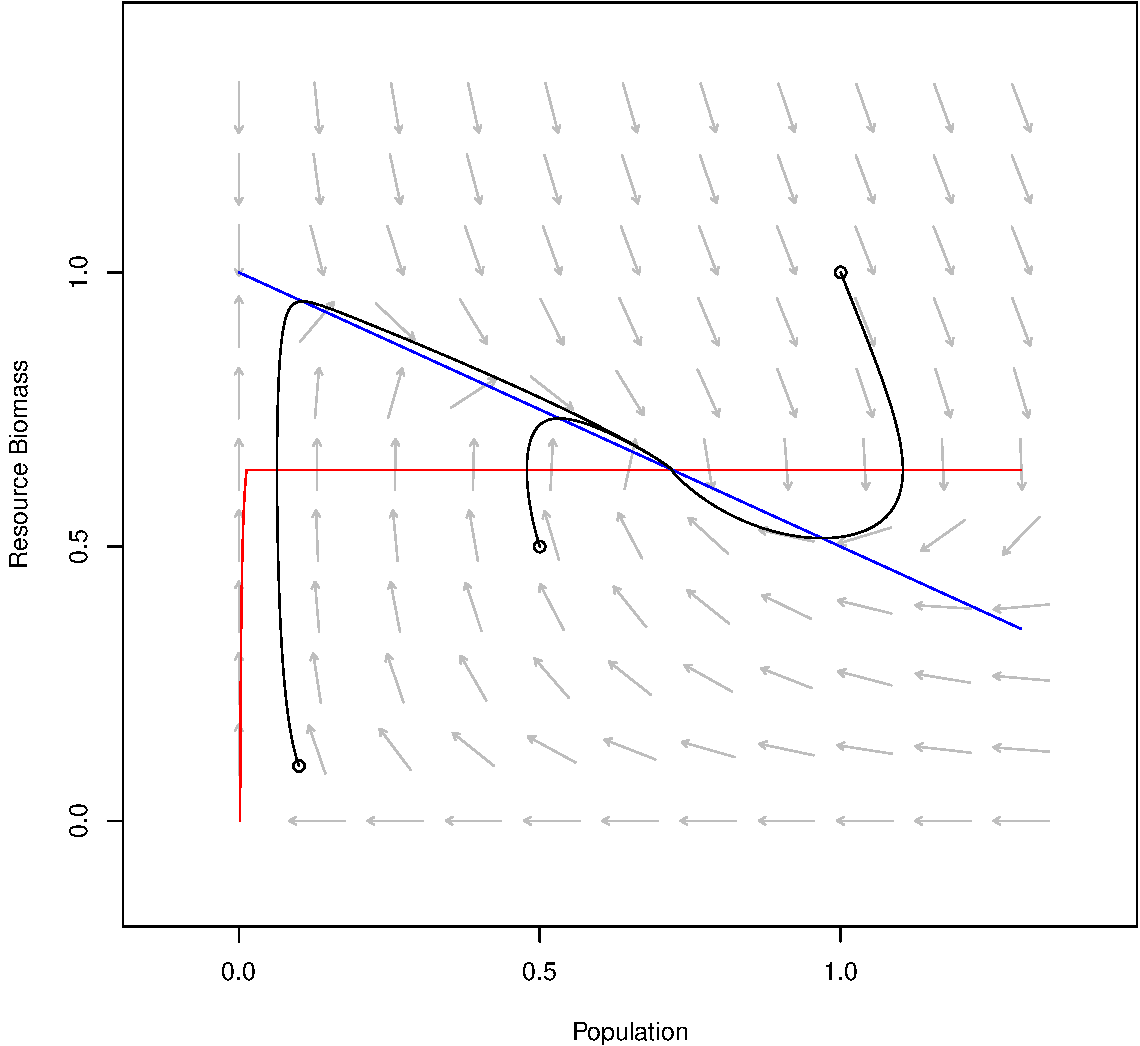
\includegraphics{consumerresource_files/figure-latex/unnamed-chunk-4-1.pdf}
Superlinear scaling of harvest ability

\begin{Shaded}
\begin{Highlighting}[]
\KeywordTok{phasePlot}\NormalTok{(netMod, }\KeywordTok{c}\NormalTok{(.}\DecValTok{5}\NormalTok{, .}\DecValTok{32}\NormalTok{, }\DecValTok{1}\NormalTok{, }\FloatTok{1.2}\NormalTok{, }\DecValTok{0}\NormalTok{, }\DecValTok{0}\NormalTok{), }\DataTypeTok{xmax =} \FloatTok{1.3}\NormalTok{, }\DataTypeTok{ymax =} \FloatTok{1.3}\NormalTok{)}
\end{Highlighting}
\end{Shaded}

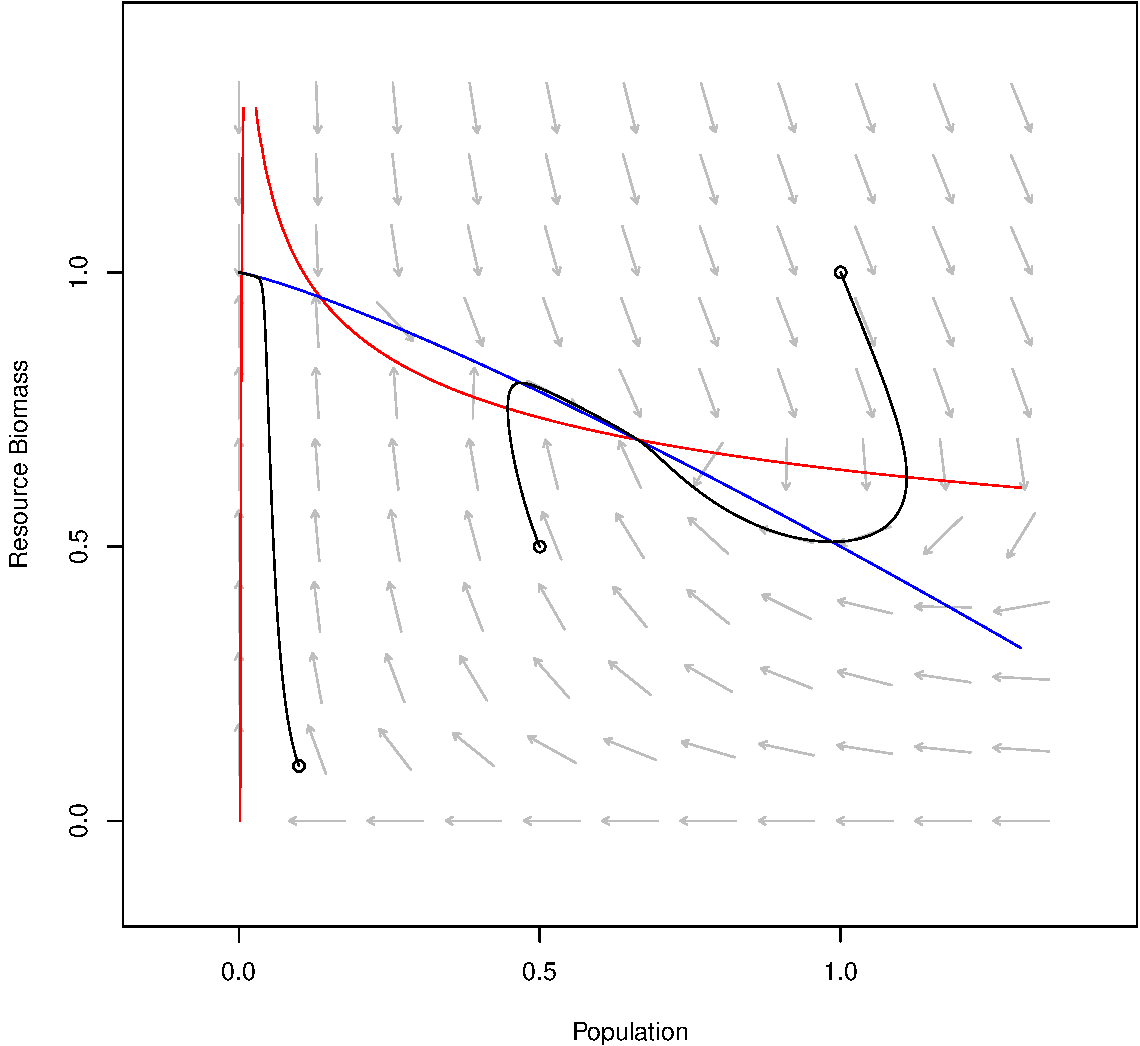
\includegraphics{consumerresource_files/figure-latex/unnamed-chunk-5-1.pdf}

Sublinear scaling of resource conversion efficiency

\begin{Shaded}
\begin{Highlighting}[]
\KeywordTok{phasePlot}\NormalTok{(netMod, }\KeywordTok{c}\NormalTok{(.}\DecValTok{5}\NormalTok{, .}\DecValTok{32}\NormalTok{, .}\DecValTok{8}\NormalTok{, }\DecValTok{1}\NormalTok{, }\DecValTok{0}\NormalTok{, }\DecValTok{0}\NormalTok{), }\DataTypeTok{xmax =} \FloatTok{1.3}\NormalTok{, }\DataTypeTok{ymax =} \FloatTok{1.3}\NormalTok{)}
\end{Highlighting}
\end{Shaded}

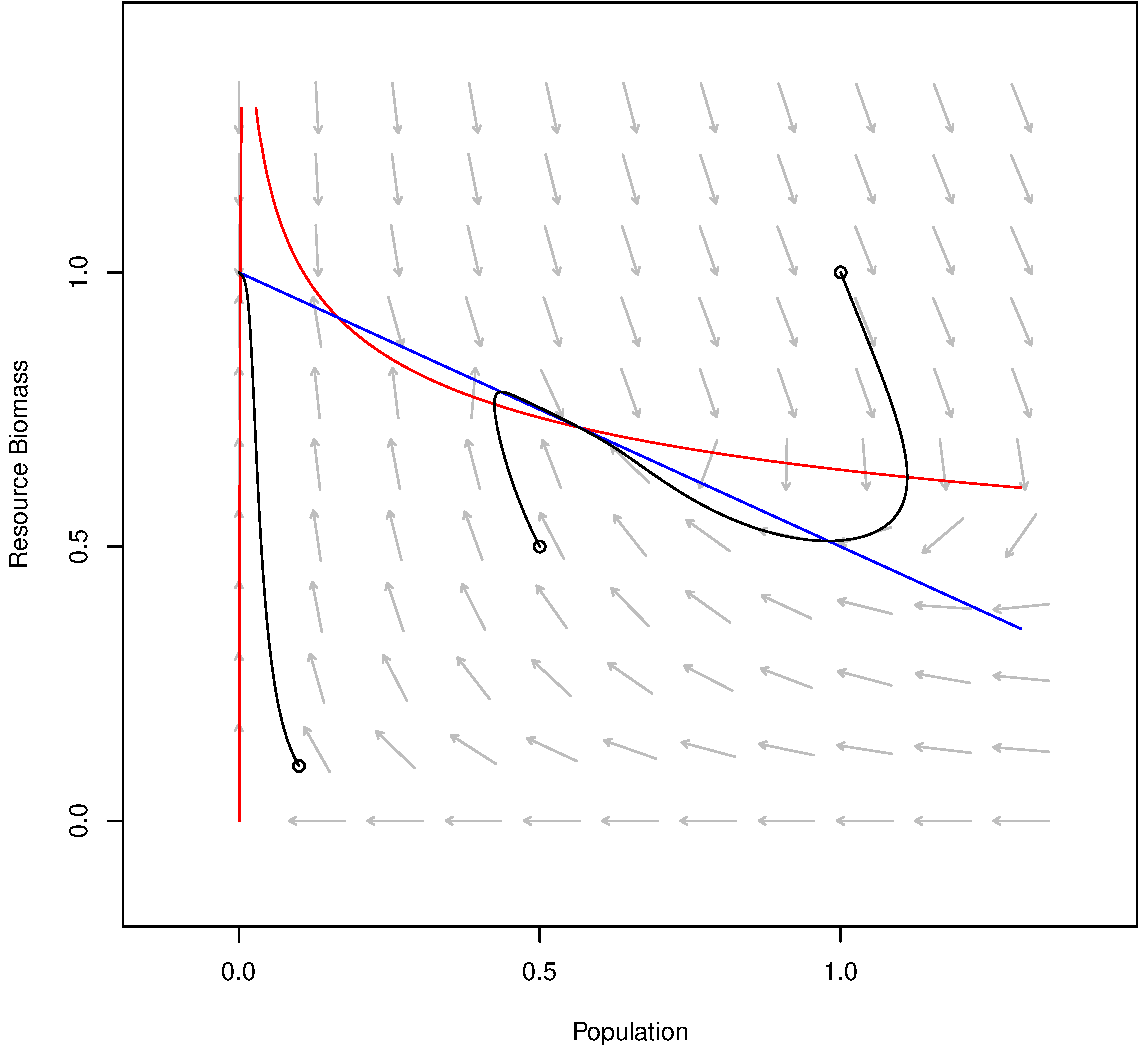
\includegraphics{consumerresource_files/figure-latex/unnamed-chunk-6-1.pdf}

Both scaling processes. lesser scaling

\begin{Shaded}
\begin{Highlighting}[]
\KeywordTok{phasePlot}\NormalTok{(netMod, }\KeywordTok{c}\NormalTok{(.}\DecValTok{5}\NormalTok{, .}\DecValTok{32}\NormalTok{, .}\DecValTok{9}\NormalTok{, }\FloatTok{1.1}\NormalTok{, }\DecValTok{0}\NormalTok{, }\DecValTok{0}\NormalTok{), }\DataTypeTok{xmax =} \FloatTok{1.3}\NormalTok{, }\DataTypeTok{ymax =} \FloatTok{1.3}\NormalTok{)}
\end{Highlighting}
\end{Shaded}

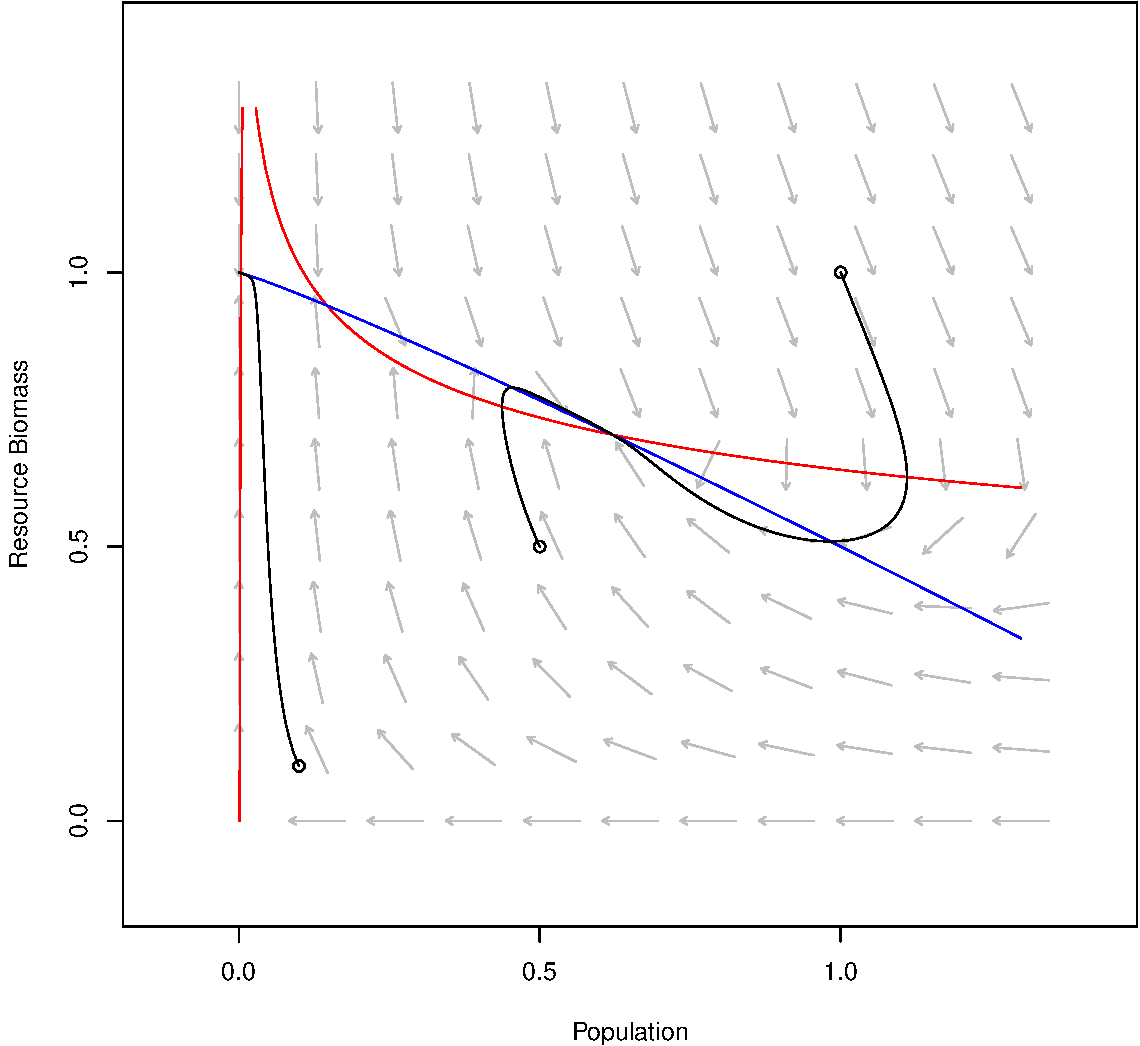
\includegraphics{consumerresource_files/figure-latex/unnamed-chunk-7-1.pdf}
greater scaling

\begin{Shaded}
\begin{Highlighting}[]
\KeywordTok{phasePlot}\NormalTok{(netMod, }\KeywordTok{c}\NormalTok{(.}\DecValTok{5}\NormalTok{, .}\DecValTok{32}\NormalTok{, .}\DecValTok{8}\NormalTok{, }\FloatTok{1.2}\NormalTok{, }\DecValTok{0}\NormalTok{, }\DecValTok{0}\NormalTok{), }\DataTypeTok{xmax =} \FloatTok{1.3}\NormalTok{, }\DataTypeTok{ymax =} \FloatTok{1.3}\NormalTok{)}
\end{Highlighting}
\end{Shaded}

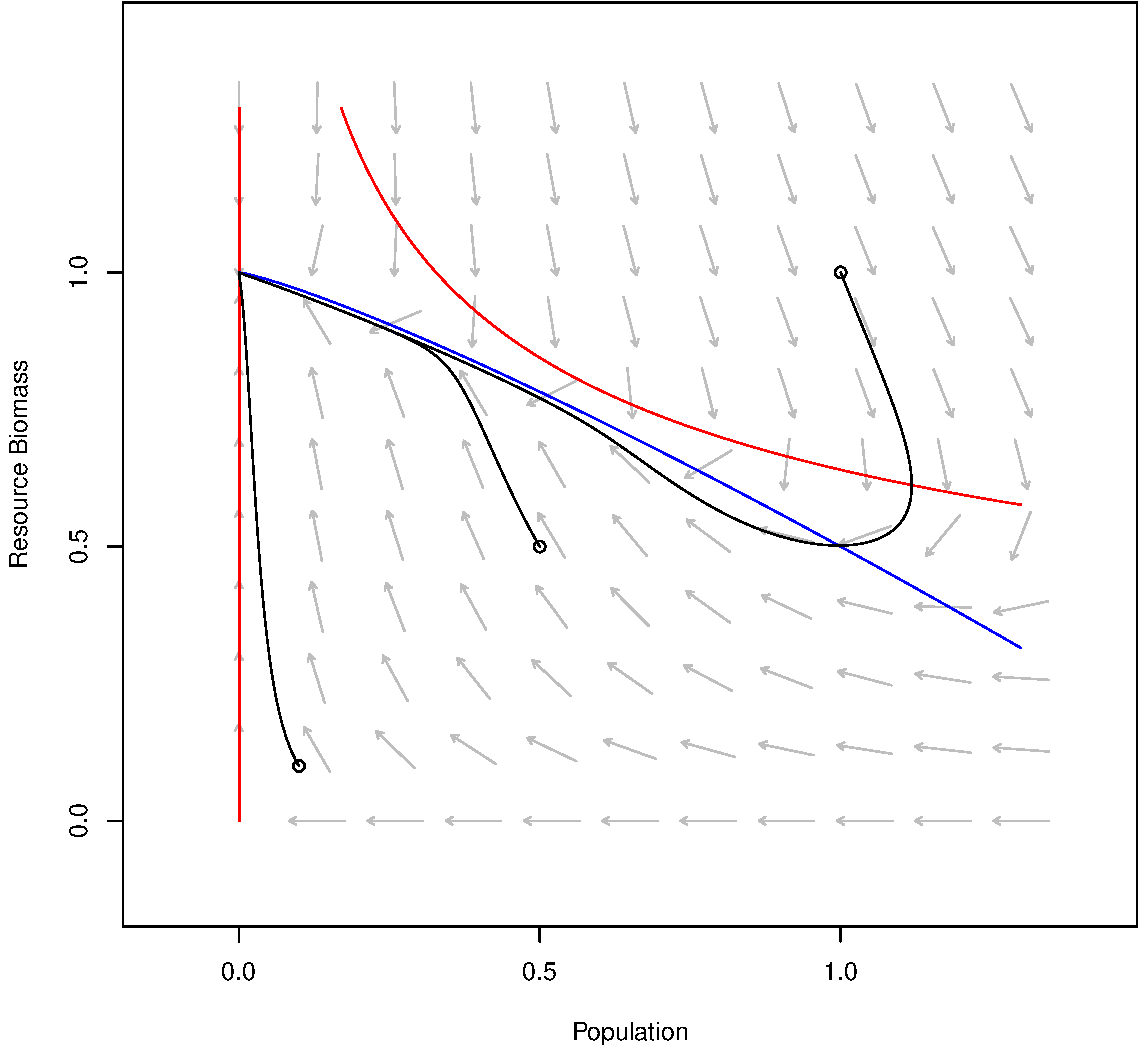
\includegraphics{consumerresource_files/figure-latex/unnamed-chunk-8-1.pdf}

\subsection{Trade}\label{trade}

\begin{Shaded}
\begin{Highlighting}[]
\KeywordTok{phasePlot}\NormalTok{(netMod, }\KeywordTok{c}\NormalTok{(.}\DecValTok{5}\NormalTok{, .}\DecValTok{32}\NormalTok{, .}\DecValTok{8}\NormalTok{, }\FloatTok{1.2}\NormalTok{, .}\DecValTok{08}\NormalTok{, }\DecValTok{0}\NormalTok{), }\DataTypeTok{xmax =} \FloatTok{1.3}\NormalTok{, }\DataTypeTok{ymax =} \FloatTok{1.3}\NormalTok{)}
\end{Highlighting}
\end{Shaded}

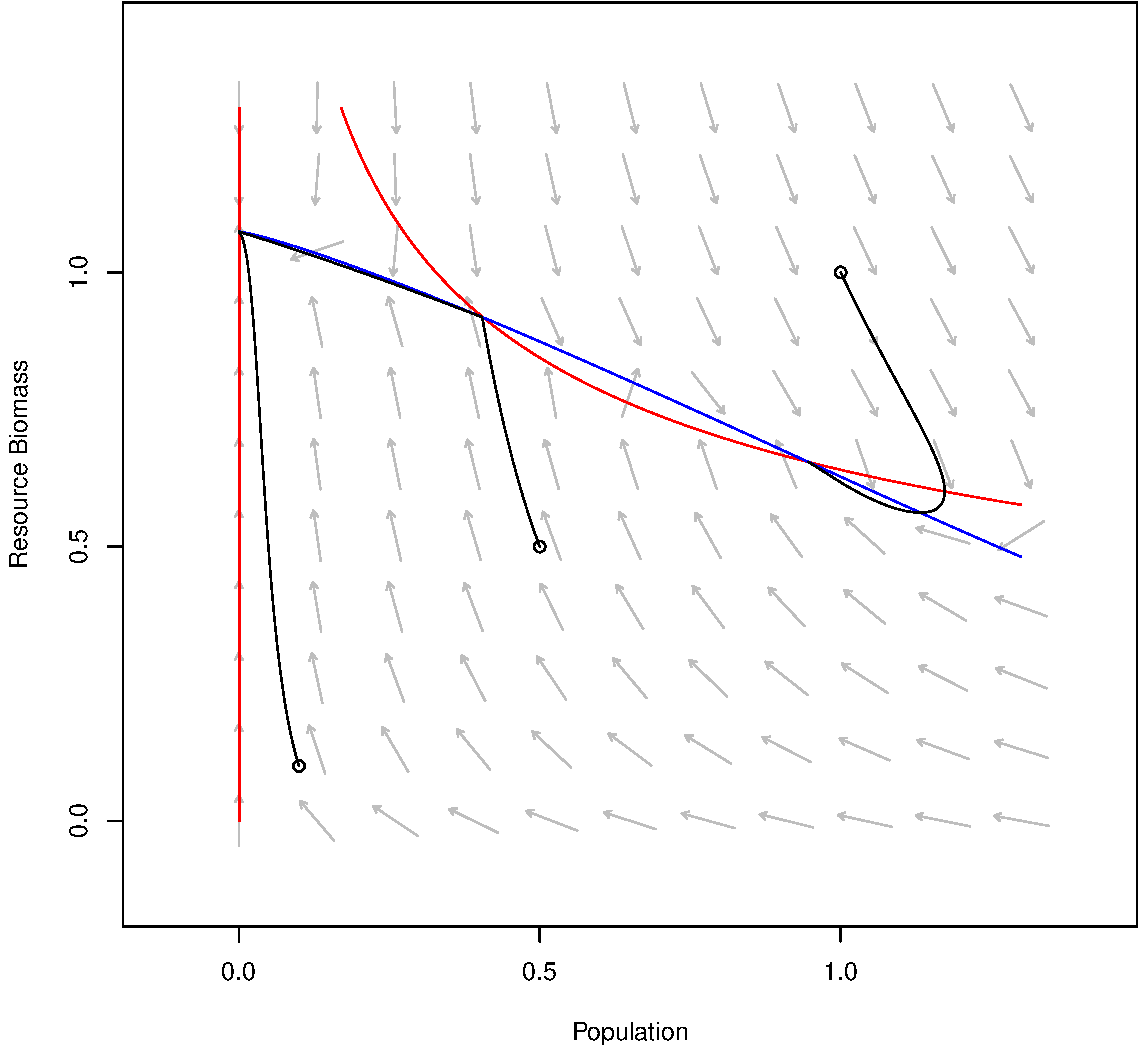
\includegraphics{consumerresource_files/figure-latex/unnamed-chunk-9-1.pdf}

\subsection{Immigration}\label{immigration}

\begin{Shaded}
\begin{Highlighting}[]
\KeywordTok{phasePlot}\NormalTok{(netMod, }\KeywordTok{c}\NormalTok{(.}\DecValTok{5}\NormalTok{, .}\DecValTok{32}\NormalTok{, .}\DecValTok{8}\NormalTok{, }\FloatTok{1.2}\NormalTok{, }\DecValTok{0}\NormalTok{, .}\DecValTok{008}\NormalTok{), }\DataTypeTok{xmax =} \FloatTok{1.3}\NormalTok{, }\DataTypeTok{ymax =} \FloatTok{1.3}\NormalTok{)}
\end{Highlighting}
\end{Shaded}

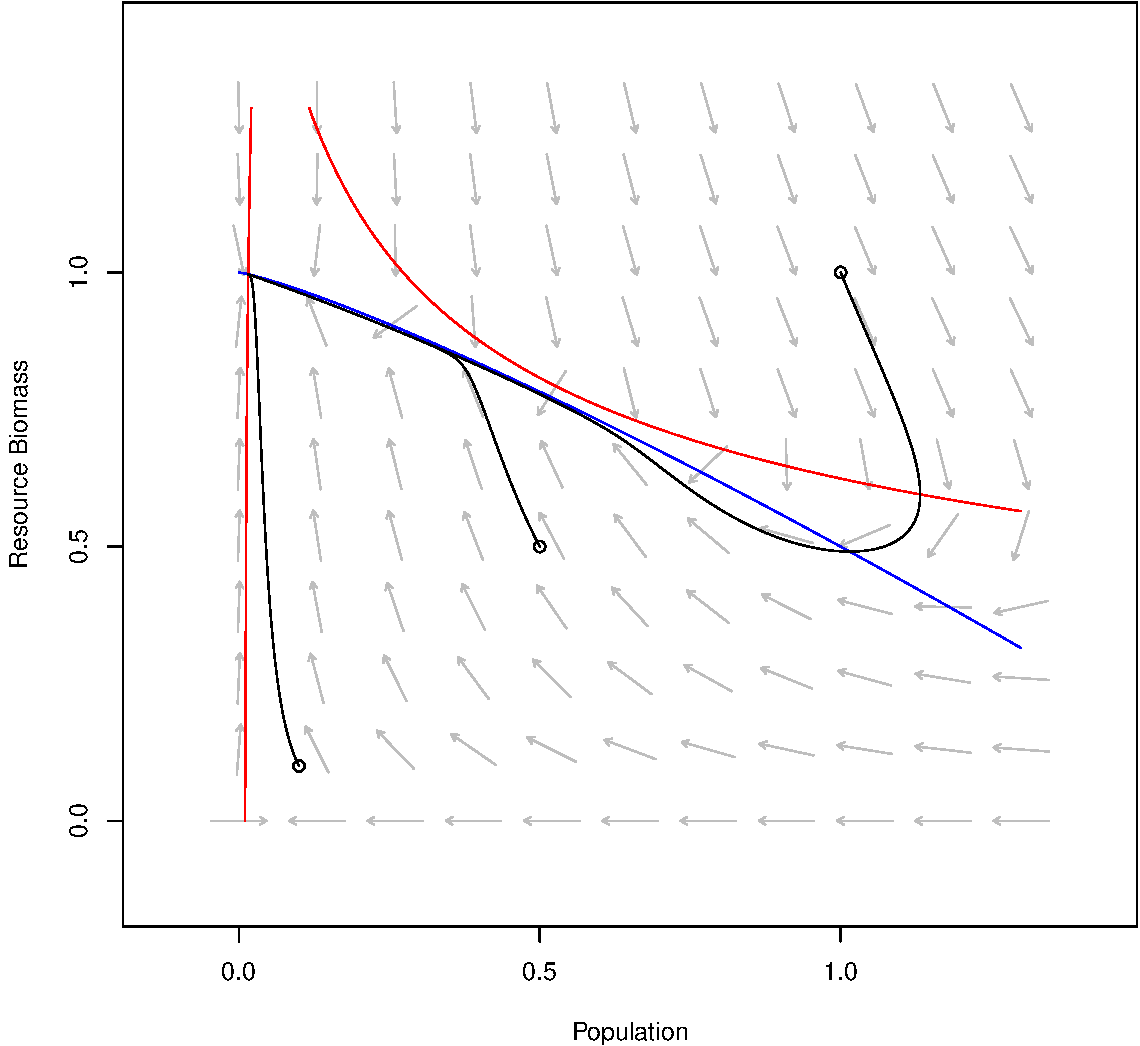
\includegraphics{consumerresource_files/figure-latex/unnamed-chunk-10-1.pdf}

\begin{Shaded}
\begin{Highlighting}[]
\KeywordTok{phasePlot}\NormalTok{(netMod, }\KeywordTok{c}\NormalTok{(.}\DecValTok{5}\NormalTok{, .}\DecValTok{32}\NormalTok{, .}\DecValTok{8}\NormalTok{, }\FloatTok{1.2}\NormalTok{, }\DecValTok{0}\NormalTok{, .}\DecValTok{02}\NormalTok{), }\DataTypeTok{xmax =} \FloatTok{1.3}\NormalTok{, }\DataTypeTok{ymax =} \FloatTok{1.3}\NormalTok{)}
\end{Highlighting}
\end{Shaded}

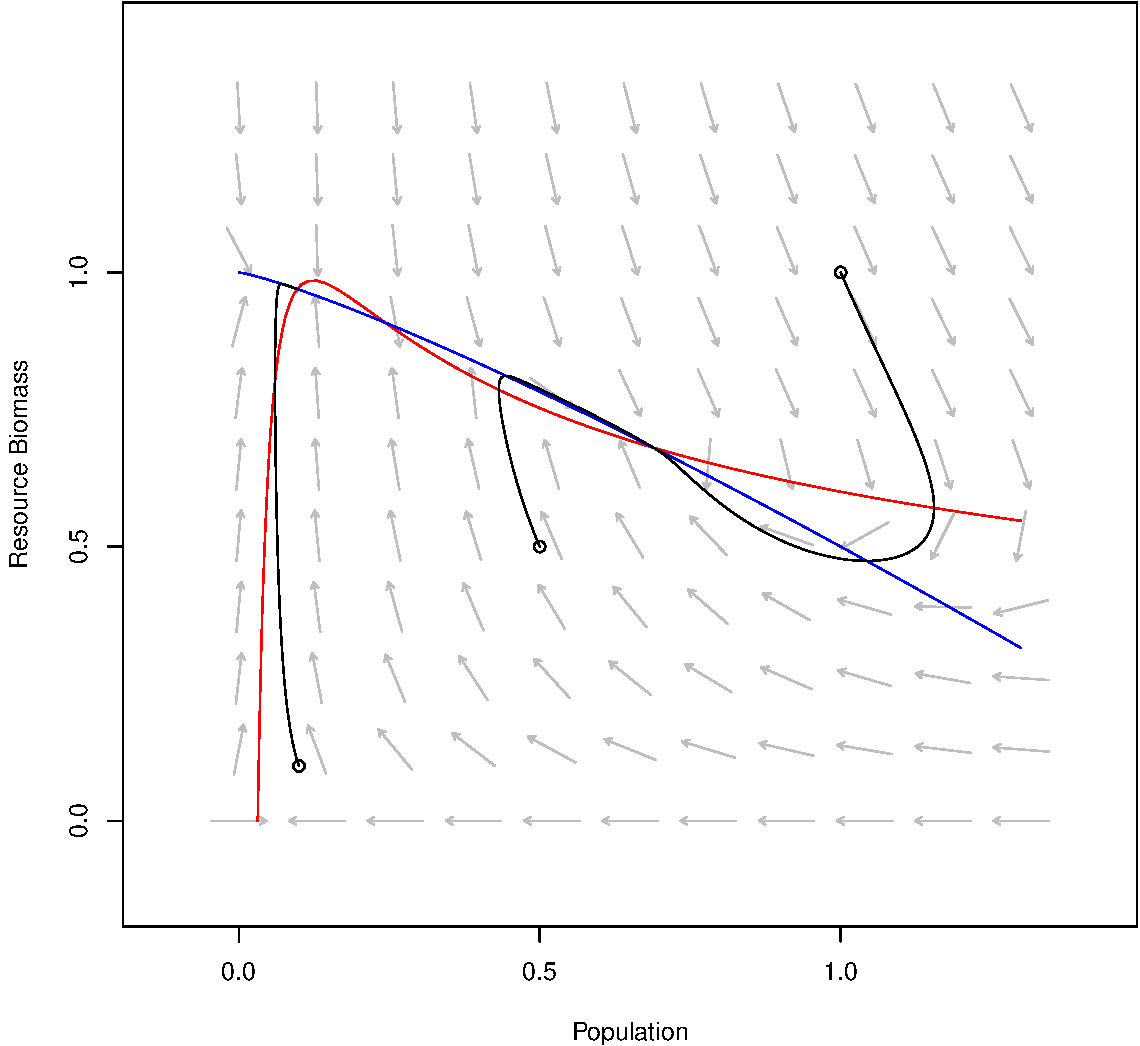
\includegraphics{consumerresource_files/figure-latex/unnamed-chunk-11-1.pdf}

\begin{Shaded}
\begin{Highlighting}[]
\KeywordTok{phasePlot}\NormalTok{(netMod, }\KeywordTok{c}\NormalTok{(.}\DecValTok{5}\NormalTok{, .}\DecValTok{32}\NormalTok{, .}\DecValTok{8}\NormalTok{, }\FloatTok{1.2}\NormalTok{, }\DecValTok{0}\NormalTok{, .}\DecValTok{03}\NormalTok{), }\DataTypeTok{xmax =} \FloatTok{1.3}\NormalTok{, }\DataTypeTok{ymax =} \FloatTok{1.3}\NormalTok{)}
\end{Highlighting}
\end{Shaded}

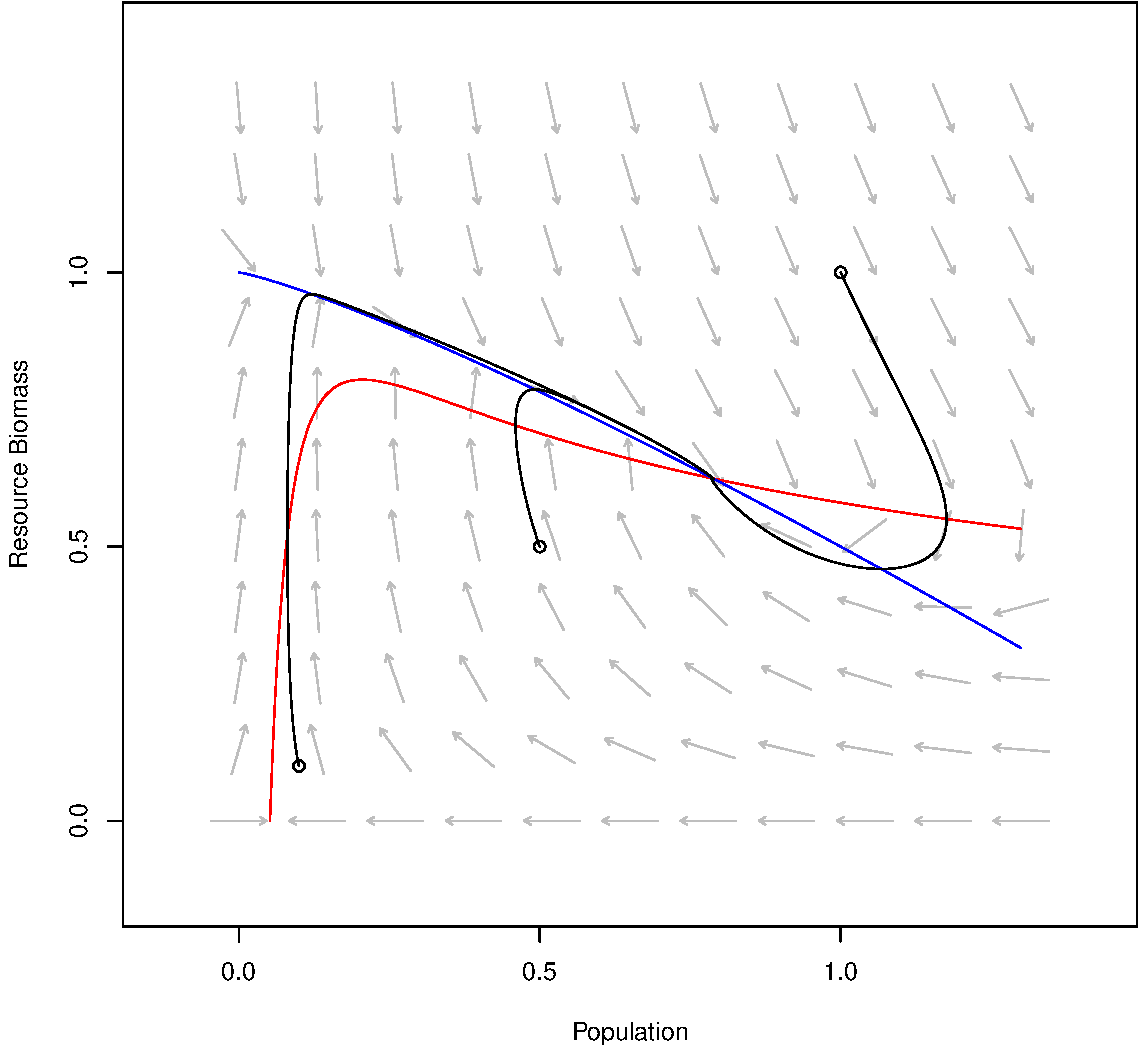
\includegraphics{consumerresource_files/figure-latex/unnamed-chunk-12-1.pdf}


\end{document}
